\documentclass[11pt]{book}
\usepackage{fontspec}
\setmainfont{TeX Gyre Pagella}
\usepackage[margin=1in]{geometry}
\usepackage{xcolor}
\usepackage{tikz}
\usetikzlibrary{arrows.meta,shapes.geometric,shapes.misc}
\usepackage{amssymb}
\usepackage{enumitem}
\usepackage{titlesec}

\titleformat{\chapter}[display]{\bfseries\Large}{Sproll 07}{0.5em}{\Huge}
\titleformat{\section}{\bfseries\large}{\thesection}{0.6em}{}

\newenvironment{algorithmproc}[1]{\vspace{0.6em}\noindent\rule{\linewidth}{0.6pt}\\[0.2em]\textbf{How to Tell: #1}\\[0.3em]}{\\[0.2em]\noindent\rule{\linewidth}{0.6pt}\vspace{0.6em}}
\newenvironment{practicenow}{\vspace{0.6em}\noindent\rule{\linewidth}{0.6pt}\\[0.2em]\textbf{Practice Now}\\[0.3em]}{\\[0.2em]\noindent\rule{\linewidth}{0.6pt}\vspace{0.6em}}
\newenvironment{exercisebox}[1]{\vspace{0.8em}\noindent\rule{\linewidth}{0.6pt}\\[0.2em]\textbf{Exercises: #1}\\[0.3em]\begin{enumerate}[label=\arabic*., itemsep=0.4em]}{\end{enumerate}\noindent\rule{\linewidth}{0.6pt}\vspace{0.6em}}
\newenvironment{trythis}{\vspace{0.6em}\noindent\rule{\linewidth}{0.6pt}\\[0.2em]\textbf{Try This}\\[0.3em]}{\\[0.2em]\noindent\rule{\linewidth}{0.6pt}\vspace{0.6em}}
\newenvironment{summarybox}{\vspace{0.6em}\noindent\rule{\linewidth}{0.6pt}\\[0.2em]\textbf{What We Learned}\\[0.3em]}{\\[0.2em]\noindent\rule{\linewidth}{0.6pt}\vspace{0.6em}}

\begin{document}
\begin{titlepage}
\centering
\vspace*{1.4in}
{\Huge \textbf{SPROLL 07}}\\[0.5in]
{\huge Same Picture, Different Story}\\[0.8in]
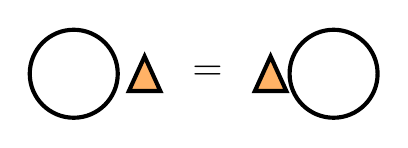
\begin{tikzpicture}
\draw[line width=1.5pt] (-1.4,0) circle (0.22in);
\draw[fill=orange!60, line width=1.5pt] (-0.7,-0.22) -- (-0.5,0.22) -- (-0.3,-0.22) -- cycle;
\node at (0.3,0) {\Large =};
\draw[fill=orange!60, line width=1.5pt] (0.9,-0.22) -- (1.1,0.22) -- (1.3,-0.22) -- cycle;
\draw[line width=1.5pt] (1.9,0) circle (0.22in);
\end{tikzpicture}\\[0.8in]
{\Large The Sproll Curriculum}\\[0.2in]
{\large Cycle I: Pops --- Things, Differences, and Counting}
\end{titlepage}

\tableofcontents

\chapter*{Before You Begin}
\addcontentsline{toc}{chapter}{Before You Begin}

This workbook does not introduce anything new. Instead, it goes back and finally answers two questions this curriculum has deliberately left open since its very first pages: whether two things that look exactly alike are really the same, and whether a picture that hides the order of events really means the order never mattered. Both questions can finally be given a precise, honest answer, now that Collapse and the idea of a chosen rule are available.

\chapter{The Two-History Question, Answered}

\section{Returning to Circle and Triangle}

Sproll 02 built two histories, circle-then-triangle and triangle-then-circle, and showed that both produced the exact same finished picture. At the time, this curriculum could only say that the picture ``forgets'' the order. Now it can say something more precise: the picture is what you get when you Collapse either history under a rule that ignores order, call it the picture rule. Both histories genuinely do collapse to the same result under that specific rule.

But recall the ledger strips from the same workbook, which did show the order clearly. Those correspond to collapsing the very same two histories under a different rule, one that keeps track of sequence, call it the sequence rule. Under the sequence rule, the two histories collapse to different results.

\begin{algorithmproc}{Same or Different, Precisely}
Two histories are equal under a stated rule exactly when collapsing each of them under that rule gives the same result. The same two histories can be equal under one rule and unequal under a different rule, and both judgments are simultaneously correct, because they are answers to different questions.
\end{algorithmproc}

\begin{exercisebox}{Section 1.1}
\item Restate, using the words ``collapse'' and ``rule,'' why the two histories from Sproll 02 could honestly be called both ``the same'' and ``different.''
\item Invent a third rule, besides the picture rule and the sequence rule, that you could apply to the circle-and-triangle histories, and say whether the two histories are equal or different under your new rule.
\item Challenge: can you think of two histories that are equal under every rule you can imagine? What would that mean about the two histories themselves?
\end{exercisebox}

\chapter{The Twins Question, Answered}

\section{Two Dots, Revisited}

Sproll 00 showed two identical-looking dots, placed apart on the page, and asked whether they were the same. That question was deliberately left open. Here is the honest answer. Under a rule that ignores position and only looks at appearance, call it the appearance rule, the two dots collapse to the same result: two circles, same size, same color. Under a rule that keeps track of position, call it the position rule, the two dots collapse to different results, because one is on the left and the other is on the right.

Neither rule is the ``real'' one. A rule that only cares what something looks like is perfectly reasonable for some purposes, and a rule that cares about position is perfectly reasonable for others. Two brand-new pennies from a coin factory are identical under an appearance rule and distinct under a position (or ownership) rule, and both facts are simultaneously true.

\begin{practicenow}
Take two identical coins or two identical sheets of blank paper. State an appearance-based rule under which they are ``the same,'' and a position- or ownership-based rule under which they are ``different.'' Confirm both rules give a sensible, correct answer.
\end{practicenow}

\begin{exercisebox}{Section 2.1}
\item Explain why ``are these the same'' was never really answerable as stated back in Sproll 00, and what question it should have been rephrased as.
\item Twins can look extremely alike under an appearance rule. Describe a rule under which two twins would clearly not be ``the same.''
\item Challenge: can you think of a rule under which two things that look completely different would count as ``the same''? (Hint: think back to the caterpillar and the butterfly.)
\end{exercisebox}

\chapter{The Group Question, Answered}

\section{One Thing or Many, Revisited}

Sproll 00 also showed a small cluster of shapes inside a drawn boundary and asked whether it was one thing or many things. This too can now be answered precisely. Under a rule that collapses everything inside a boundary into a single unit, call it the boundary rule, the cluster is one thing. Under a rule that looks past the boundary and counts each individual mark, call it the parts rule, the same cluster is several things. Both are legitimate collapses of the exact same picture, using different rules.

\begin{summarybox}
A question like ``are these the same'' or ``is this one thing or many'' is incomplete as stated. The complete, answerable version always names a rule: ``are these the same under this rule.'' Two things can honestly be the same under one rule and different under another, without any contradiction, because each judgment is a separate, correctly answered question.
\end{summarybox}

\begin{exercisebox}{Section 3.1}
\item Using the pennies-and-dollar example from Sproll 00, state the two rules involved explicitly, in the vocabulary of this workbook.
\item Take any object made of multiple parts near you (a book with pages, a sandwich with ingredients) and state one rule under which it is one thing and one rule under which it is many things.
\item Challenge: is there ever a case where a question like ``is this one thing or many'' genuinely has no sensible rule that would answer it clearly either way? Try to think of an example.
\end{exercisebox}

\chapter*{Looking Ahead}
\addcontentsline{toc}{chapter}{Looking Ahead}

If sameness always depends on a chosen rule, is there a way to be careful and precise about exactly when two things should be called equal, rather than relying on a loose sense of ``looks the same''? That is the subject of the next workbook, Sproll 08: When Are They Equal?

\chapter*{For Parents and Teachers}
\addcontentsline{toc}{chapter}{For Parents and Teachers}

This workbook resolves, rather than merely revisits, the two open questions left standing since Sproll 00 and Sproll 02. Both resolutions depend on Collapse (Sproll 06) being fully available, and both are stated in this curriculum's technical companion material as instances of a single formal principle: historical identity, and identity of appearance more generally, is always relative to an observation rule, never assumed from the syntactic or visual form of what is being compared. This workbook is where a child sees that principle pay off directly on two questions they were asked to sit with, unresolved, several workbooks earlier.

\end{document}
